\chapter{Existing solutions}\label{chapter:research}

There are many existing game engines, and I think it is important for me to examine where they succeed and where they fail so I can learn from them. Sadly, as I have mentioned, there aren't many engines that we can use for free, and there are even fewer engines where we can see the source code as well. In this section I will be presenting a few of the existing engines and what I think their strong points and mistakes are.
As I have the most experience with Unity I will be exploring it in more detail than the others.


\section{Unity}

The Unity game engine\cite{unity}, developed by Unity Technologies, is an extensive platform known for creating many types of interactive content, with a primary emphasis on video games, but it is also used in simulations or architectural visualization. This engine allows the creation of 2D, 3D, and virtual reality (VR) games for almost every platform, such as Windows, macOS, Linux, Mobile, and consoles. Unity rose in popularity due to its cross-platform capabilities, easy to use environment, and the supportive community that formed around it. It uses \Csh as the primary scripting language, which is known for its versatility and efficiency, this also made it popular among developers. Additionally, its intuitive design and the availability of extensive learning resources have made Unity highly accessible, propelling its popularity.

In Unity, the game's world - called Scene - is built from Game Objects, which can represent anything that is necessary for the gameplay. Most commonly these include the player and the environment they are in, but can also be more abstract things like managers for different game systems. To give these Game Objects logic, the user needs to add Components to them. One of the most common components are Mesh and Mesh Renderer which make the Game Object show up in the game world. The engine has many other built in components that can add physics, rendering, sound and many other capabilities to the objects. If the built-in set of components are not enough, than the user can create custom components by writing \Csh scripts that extend the \verb|MonoBehaviour| base class. The game objects can be attached to each other called "parenting", this causes them to move together with the parent object. This is commonly used to make a camera or a clothes follow the player.

These scenes are authored inside the editor using the Scene view, Hierarchy, and Inspector sections. In the scene view, we have a bird's eye view of the environment we are creating, while the Hierarchy and Inspector views provide a more abstract way of editing the scene. The Hierarchy (\autoref{fig:unity-hierarchy}) shows a list of all the Game Objects that are present in the scene, because these can have parent-children relations this view forms a tree.

Inspector (\autoref{fig:unity-inspector}) is a view that shows the properties of the currently selected object. This view is used to edit the properties of the Game Object, the Components attached to it, and to add new components to it.

Despite Unity's popularity in the independent developer community (called "indie" developers) and huge success in creating diverse games, it is not without shortcomings. One of the most glaring issues I have encountered have been with the sporadic updates. Unity seams to be focused on chasing the newest and most cutting edge technologies, but this often results in a neglect of existing bugs and stability issues. As a long time user, it feels like the engine has become more and more cluttered with new half finished features, and even more bugs. Many of the new features announced years ago are still in development, and many others have been silently discontinued.

Because of this constant chase of the new technologies, there are many areas where multiple competing solutions exist for a single problem. The most infamous example is the networking libraries, where there are multiple solutions. These make the developer's choice for what system to use harder, as older solution might be unsupported in the next engine version, but the replacement is not yet ready in the current version. This makes even starting a new project really hard and require a lot of unnecessary decisions.

\begin{figure}[h]
    \centering
    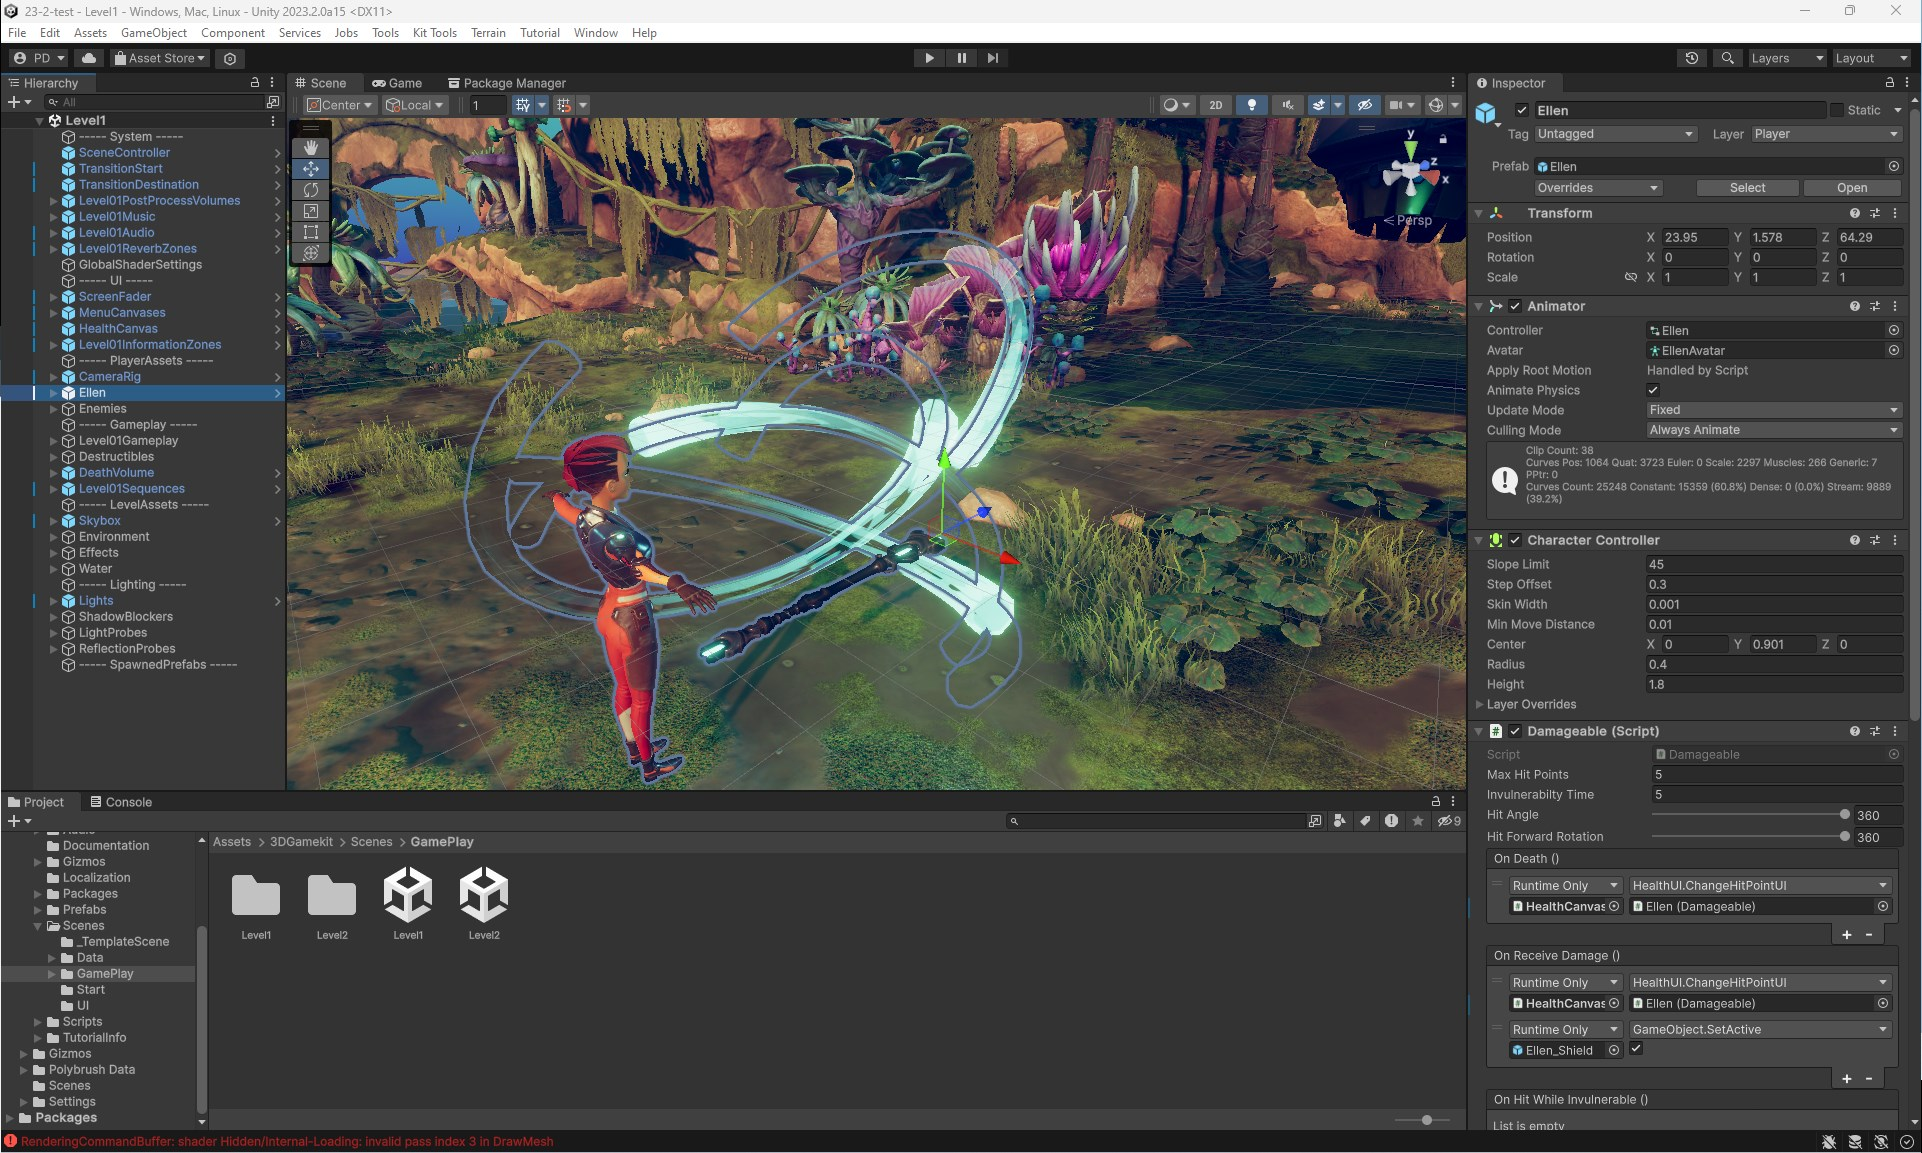
\includegraphics[width=\textwidth]{content/Research/Unity-Editor-2.jpg}
    \caption{Screenshot of the Unity engine's unified editor.}
    \label{fig:unity-editor}
\end{figure}


\section{Unreal Engine 5}

Unreal Engine (UE), developed by Epic Games, has a rich and long history that has significantly influenced the landscape of modern gaming. The inception of Unreal Engine dates back to 1998, when the first-person shooter game 'Unreal'\cite{unreal-game} was released. Since then, it has undergone several mayor transformations, resulting in its latest iteration Unreal Engine 5 (UE5). Throughout the years, the engine has consistently pushed the boundaries of what's possible in game development, from pioneering high-fidelity graphics to realizing expansive virtual worlds.

Unreal Engine 5, boasts a tremendous leap forward in visual fidelity, by using groundbreaking technologies such as Nanite and Lumen.
Nanite is a system that essentially eliminates the limitations of polygon count and draw call overheads in 3D environment modelling. It achieves this by using so-called "virtual polygons", allowing for much greater model detail to be used without major performance hit. This system can replace the traditional Level Of Detail (LOD)\footnote{A system where separate models are created for when the given object is further away.} approach, allowing for much faster development time.
Lumen, on the other hand, is a fully dynamic global illumination solution that can immediately react to scene and light changes, producing more lifelike environments. It is important to highlight that while these technologies can produce stunning visuals, they are slower than traditional approaches and not suitable for every game, or platform.


\begin{figure}[h]
    \centering
    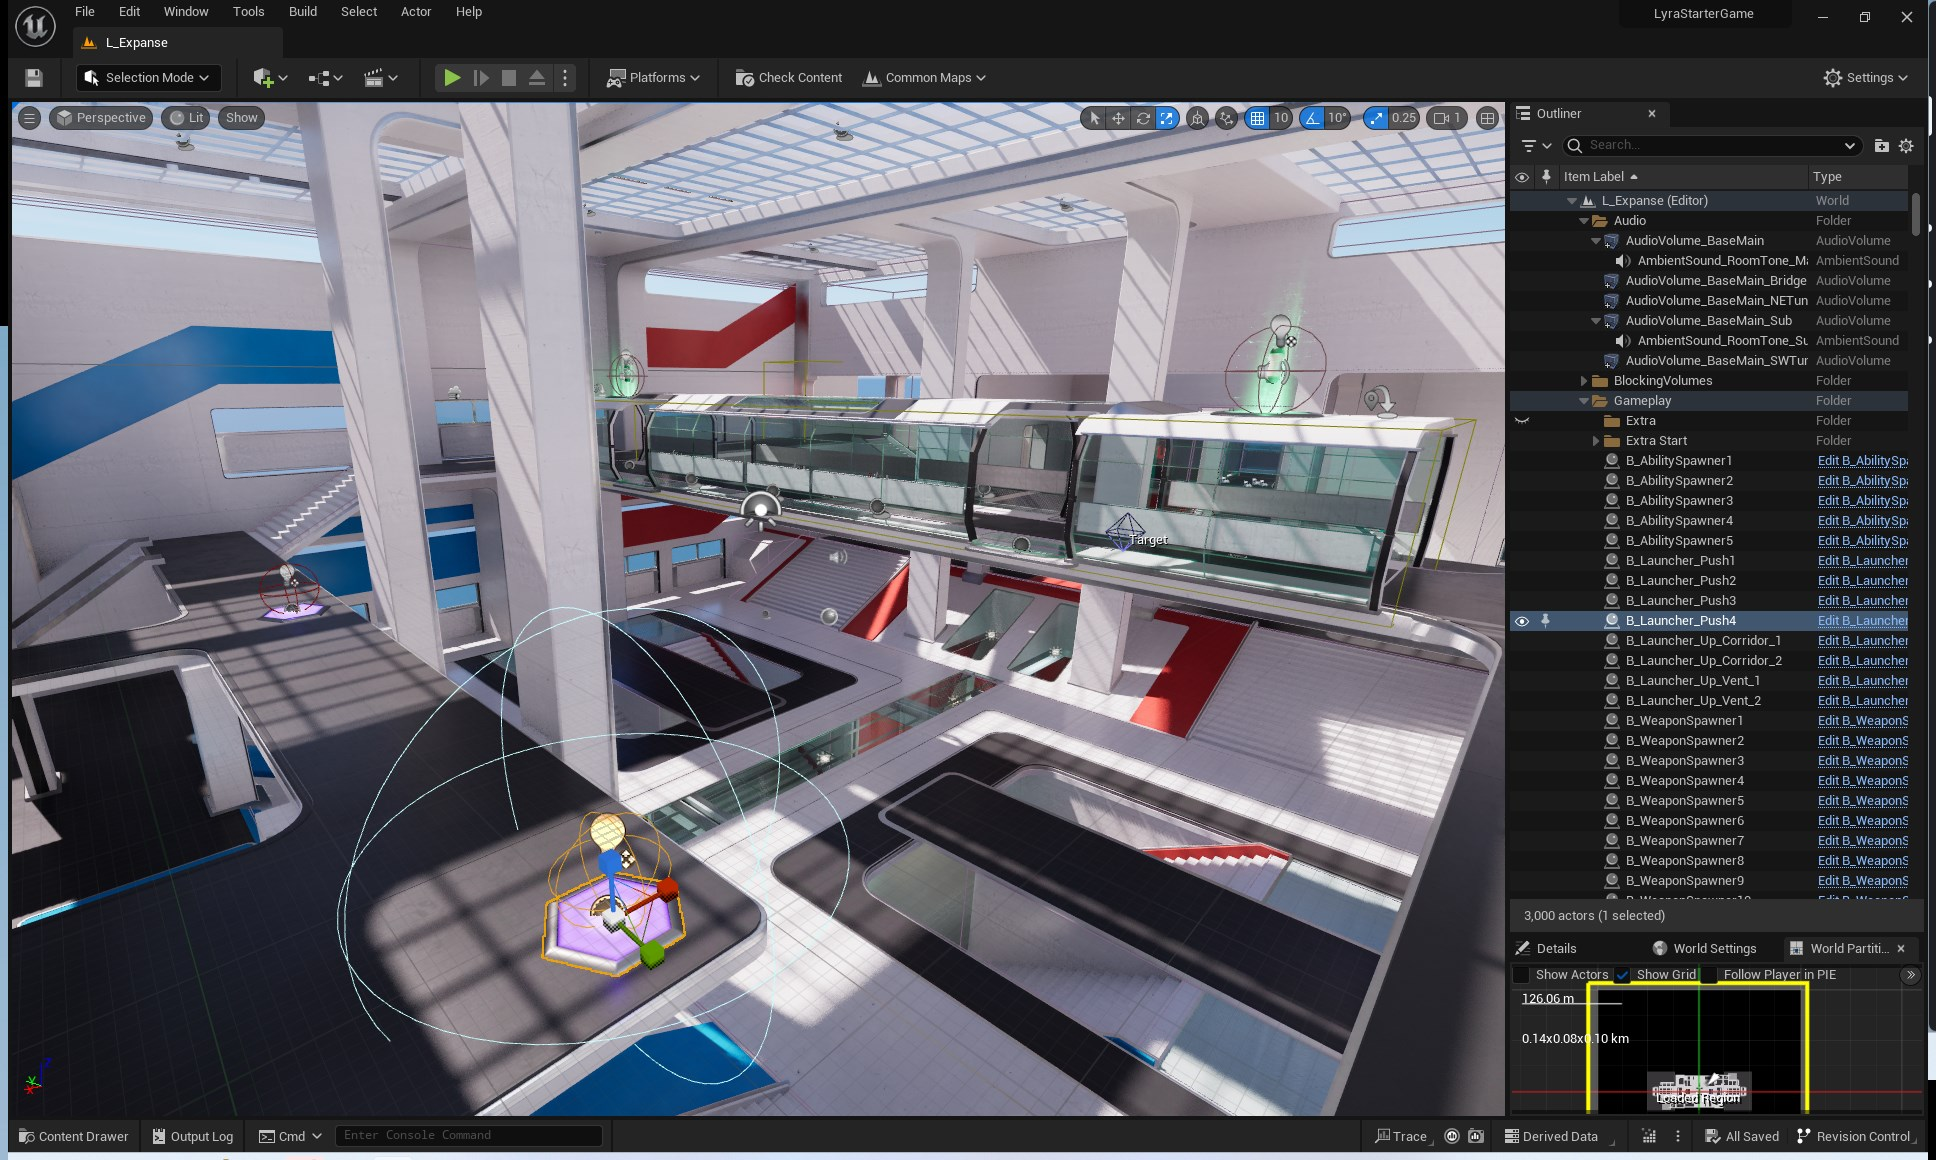
\includegraphics[width=0.8\textwidth]{content/Research/UE5-editor}
    \caption{Screenshot of the Unreal Engine 5 editor.}
    \label{fig:ue5-editor}
\end{figure}

\subsection{Actors and the Outliner}

In UE 5, the fundamental building blocks of a game world are called Actors. An Actor is essentially any object that can be placed into the game world, and they can represent characters, scenery, and even complex gameplay elements. There are many built in Actors that do common functionality, for example common game objects such as characters, cameras, lights, and physics objects.

The list of the Actors present in the game world is shown in the Outliner witch is a tool within UE5 editor that provides a hierarchical view of all the Actors present in a level (\autoref{fig:ue5-outliner}).

Components are the building blocks of Actors, and they can be thought of as the individual features that make up an Actor. For example, a character Actor might have a Mesh Component, a Camera Component, and a Character Movement Component. Components can form a parent-child relationship inside an Actor. This allows for the creation of complex Actors. The list of components present in an Actor is shown in the Details panel (\autoref{fig:ue5-details}), this shows the hierarchy of the components and their properties.

But the user also has multiple options to create new types specific to their game. One such method is through the use of Blueprints, a visual scripting system that allows for the creation of custom Actors without the need for traditional programming. This system uses visual nodes to define the code flow, and is quite beginner-friendly. By combining pre-existing components and defining their interactions through Blueprint nodes, developers can create new Actor types that fit their game's requirements.

Another method for creating new Actor types is through \Cpp programming.
UE5 is written in \Cpp and natively only supports \Cpp based scripting, but plugins exist which allow for other languages like \Csh to be used for coding. These methods are more complex and requires a good understanding of \Cpp and the UE5 API, but it allows for more advanced functionality and performance optimizations.

